\section{Attack setup}
In all our complete attacks except one, we attacked a Linux machine running Ubuntu Server 15.10 (Linux kernel 4.2) with Intel VT-d as the IOMMU, a Broadcom NetXtreme II BCM5709 Gigabit Ethernet and Mellnox ConnectX-5 100GbE as the network controllers. In later experiments, we used newer versions of Ubuntu (16.04,17.10,18.4) \textcolor{red}{but did not implement a complete attack against these versions - Any need to be explicit about it?}. An identical machine that was connected to the victim machine with a FireWire cable simulated the attacker. In our final experiment, we attacked FreeBSD 10.3 running on the same hardware.  Linux kernel supports emulating hard disks for remote computers, which is implemented in the Linux-IO Target (LIO) subsystem. We modified the login function of the SBP-2 disk emulator on the attacking machine to invoke the attack, in addition to its normal work, whenever we wanted to attack using a physical device.To attack a physical machine using an unmodified network card, we used a FireWire device in a similar technique to the one used by Sang et al. \cite{SLND10}: by carefully modifying the victim’s OS, we forced it to believe that the network card and the FireWire device were actually the same device (PCI aliases), and made them use the same IOVA page tables. In this way, we could attack using a programmable interface without having to modify the real attacking device, which, in general, is much harder.
\subsection{Linux FireWire} \label{sec:sbp2_attack}
\begin{figure}
    \centering
    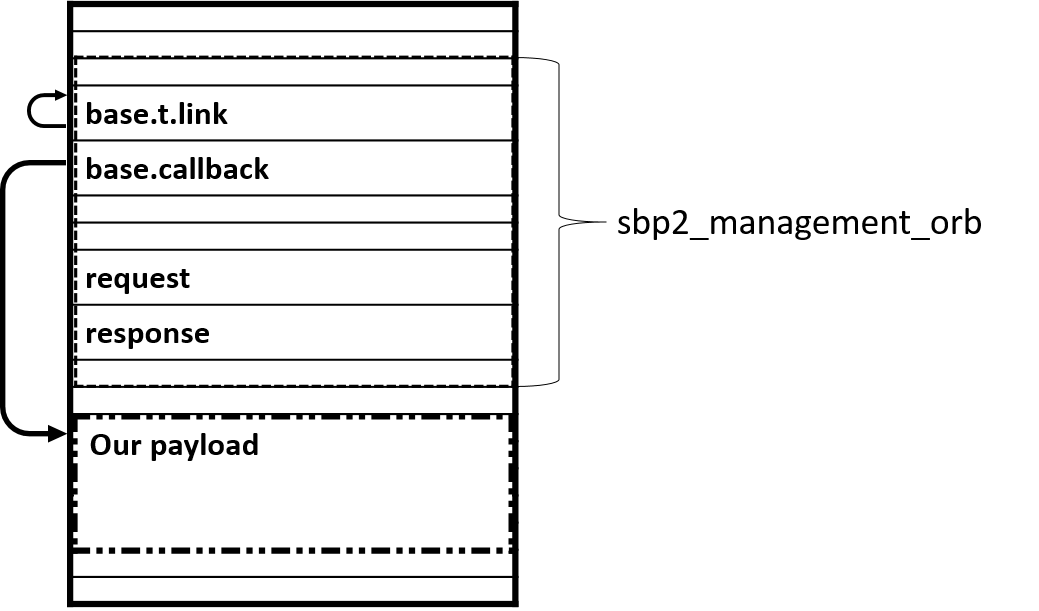
\includegraphics[width=1.1\linewidth]{figs/sbp.png}
    \caption{Caption}
    \label{fig:orb}
\end{figure}
We found that the Linux FireWire driver has a deterministic sub-page granularity vulnerability. The device data resides on the same page with driver metadata; providing both \means and \oportunity .\newline
To connect to a target, the initiator sends a login request. When the target is ready, it fills the buffer that was pointed to by the request with a login response(shown in Figure \ref{fig:orb}) using DMA, and reports to the initiator that it has done so. In Linux’s SBP-2 driver, management ORBs, and the login ORB in particular, are represented by the sbp2 management orb data structure. This data structure holds the buffers for the request and the response, as well as other fields necessary for the communication. The fields that are relevant for the attack are shown in Figure \ref{fig:orb}. In order to enable the communication, the driver maps the request and response fields in sbp2 management orb for read and write by the device, respectively. As a result, the device has the same 4k page accessible to read using the \iova that was created when the request was mapped and accessible to write via the \iova created when the response on the same page was mapped. Now this page is entirely visible to the device both for reading and writing; consequently, the device is able to read and manipulate both the request/response fields and the metadata that controls the CPUs behavior. Sbp2 management orb contains a callback function, \texttt{base.callback}, that is invoked after the target has responded. By overriding the callback pointer, attackers can run arbitrary code in the kernel context. We note that in the general case, the original callback must be called before/after the attack code, so the device behavior will not break. In this specific case, however, we saw that the original callback creates no actual side effects and could be ignored. Now, the attacker needs to bring the shellcode\footnote{The entire shellcode appears in Appendix \ref{apx:shellcode}.} into the victim’s memory and point to it using a kernel virtual address. We put the shellcode in the same already device-writable page. The device has the correct \kva from reading the \texttt{base.t.link} field.  This field is used in lower level transactions of FireWire and is guaranteed to point to itself when the target receives the request (i.e., when we attack); KASLR is broken with this pointer and is not a hurdle in this attack. In this scenario the \kva to the shellcode and and the callback were provided readily by the \spb2 protocol implementation. Attaching a malicious FireWire device was enough to take over the machine regardless of IOMMU and KASLR. 

\begin{comment}
In fact, in the basic attack, the shellcode was small enough to fit into the unused space between the sbp2 management orb structure and the end of the slub object (whose size is always a power of two). In later versions of the payload, we manipulated the memory allocator’s freelist in order to make room for the attack payload. The last field we used in sbp2 management orb is \textit{base.t.link}.  By reading this pointer, the attacker is able to deduce the shellcode’s virtual address and set it into callback to launch the attack. Reading the kva directly from sbp2 management orb, however, works better and is more robust.
\end{comment}
\begin{comment}


\subsection{FreeBSD UMA}
\textcolor{red}{This is way to close to what the NDSS paper did...}
We use FireWire to target the FreeBSD Universal Memory Allocator(UMA). By attacking the kernel memory allocator rather than the driver of a specific device, we demonstrate that the problem is not unique to buggy drivers. Saving metadata that is related to the memory management within a data page is a common method for memory allocators and we show that this is a dangerous practice \cite{Cor07, ak09}. FreeBSD is somewhat simpler because its memory maps are always both for reading and writing by the device. UMA is the memory allocator that the FreeBSD kernel uses internally for it own memory allocations. In order to not waste more memory than it has to, UMA saves some management metadata in a structure within data pages when possible (e.g., when the size of the objects is small enough); otherwise, it saves all the management metadata off-page. Inspired by the way Argp and Karl attacked the UMA in an earlier version of FreeBSD (using a regular heap-overflow vulnerability in a sample module) \cite{ak09}, we overrode this metadata, successfully gaining code execution with kernel context. The attack is not unique to the FireWire driver and is applicable to any driver that maps a small variable allocated using UMA. During the initialization of FreeBSD’s FireWire driver, it allocates a dummy ORB that is sometimes required according to SBP-2 protocol. As a result, there is a 4-byte integer that is always allocated using UMA and is mapped at a fixed IOVA. Since UMA saves the metadata of pages with 4-byte objects on-page, it is accessible by the device. This metadata structure contains pointers to other structures with a few levels of indirection; one of them contains several pointers to functions. In particular, we used a destructor that UMA calls during object freeing\footnote{\textcolor{red}{Need to show the data structures and ptrs}}. The specific hierarchy is inherited from the UMA design, and can be found in \cite{aA10}. Using these metadata structures, we implemented a proof of concept by overriding only the necessary pointers to finally get the destructor points to an address in the same mapped page and set a simple payload there that is built only from int3 (debugger break-point opcode)\footnote{\textcolor{red}{Wouldnt be better just to say thast we put our payload there? - Why say we did less?}}. As we did for the Linux FireWire attack, we got the virtual address of the page—which we needed for setting up the pointers—from the us data field in the original metadata structure. This address points to the first item in the slab. \textcolor{red}{When we disabled standard kernel protections - Did what? Is an attack feasible?}, we successfully got an unexpected break-point error.
\end{comment}